% Wspólna okładka A4: kreskówkowa scena z wkomponowanymi napisami.
\documentclass[tikz,border=0pt]{standalone}
\usepackage{graphicx}
\begin{document}
% Odpowiednik tekstowy napisów dla kopiowania i czytników PDF.
\pdfliteral direct {/Span << /ActualText <FEFF00540065006F0072006900610020006D0069006100720079002E0020005A0061006B0142006100640061006D007900200041004B0053004A004F004D004100540020005700590042004F00520055003F0021002000500052005A00450053004100440041002E0020004A0061006B002000740065006E0020004100530020005700590057004900410044005500200074006F002000770073007A007900730074006B006F0020007700690064007A0069003F0020004B0061017C0064007900200063007A00770061007200740065006B00200074006F0020007000610072007A007900730074007900200063007A00770061007200740065006B002E002000500052004100570044005A004900570045002003C3002D0043004900410141004F002E> >> BDC}
\begin{tikzpicture}[x=1mm,y=1mm,every node/.style={inner sep=0pt}]
  \path[use as bounding box] (0,0) rectangle (210,297);
  \node[anchor=south west] at (0,0)
    {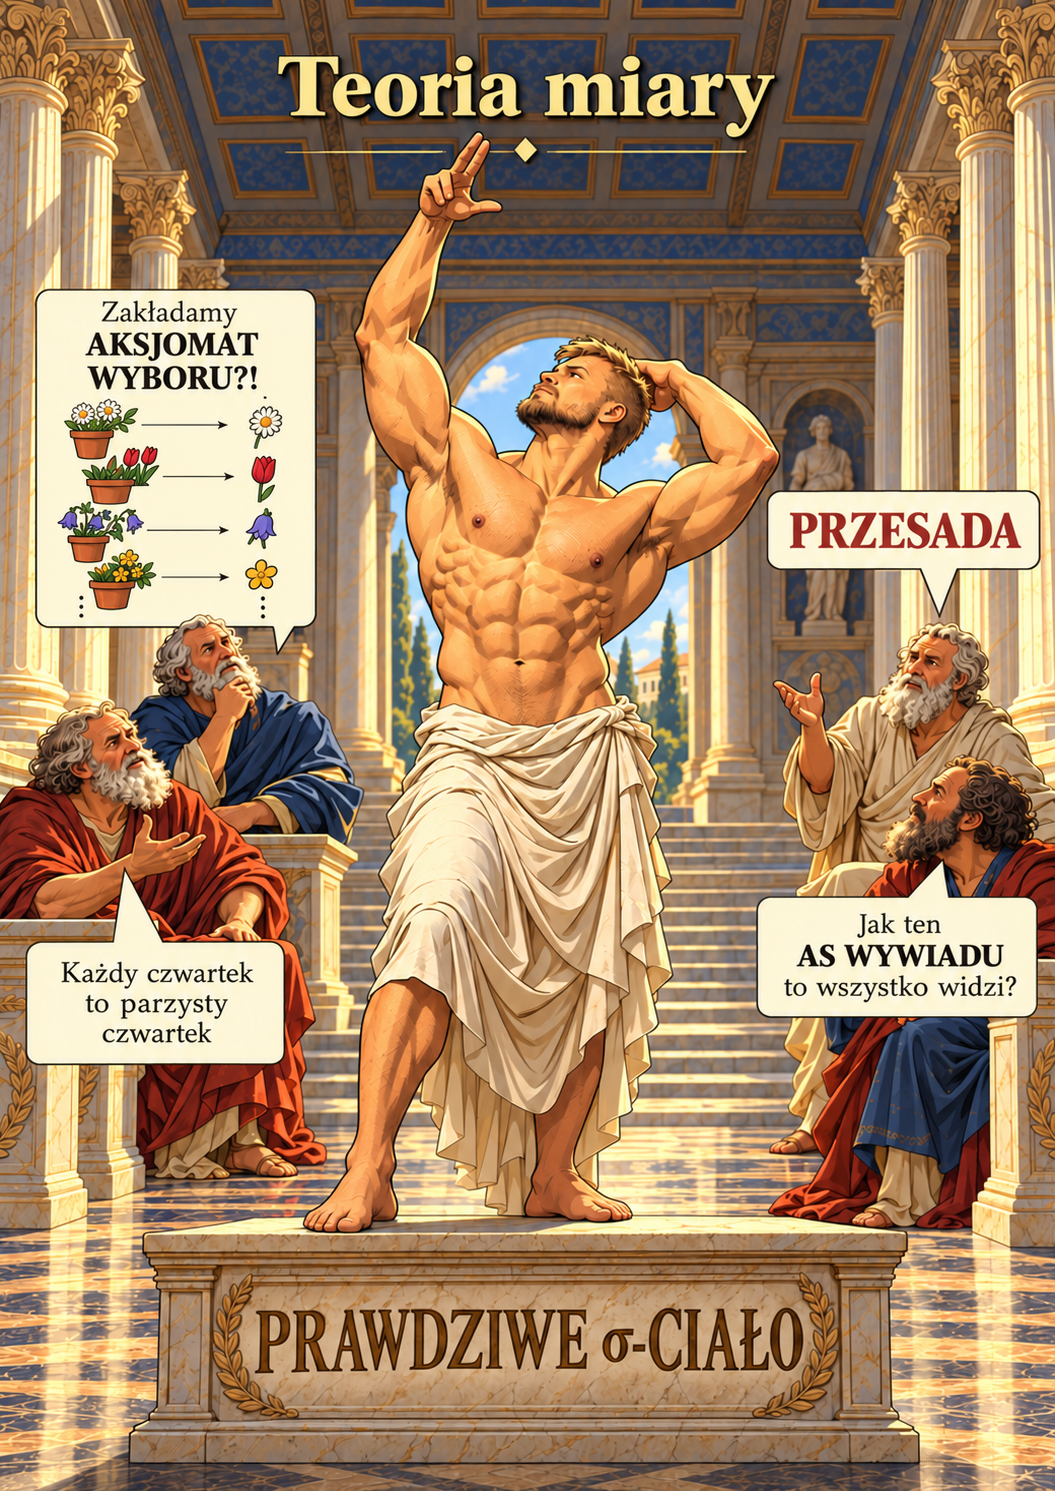
\includegraphics[width=210mm,height=297mm]{okladka-kreskowkowa.png}};
\end{tikzpicture}
\pdfliteral direct {EMC}
\end{document}
